\chapter{Challenge II}
\section{Outline}
\begin{enumerate}
   \item Each subject manages a list with its own capabilities
   
   \item The operation field of a capability is encrypted with a key private to the security kernel SK
   
   \item To request operation Op on object O, a subject S sends to SK a message with S, O, Op and the encrypted capability
   
   \item SK decrypts the capability and, if it enables Op on O, it asks O to create a channel with S to execute OP
   
   \item O destroys the channel when Op ends
\end{enumerate}

\begin{figure}[htbp]
   \centering
   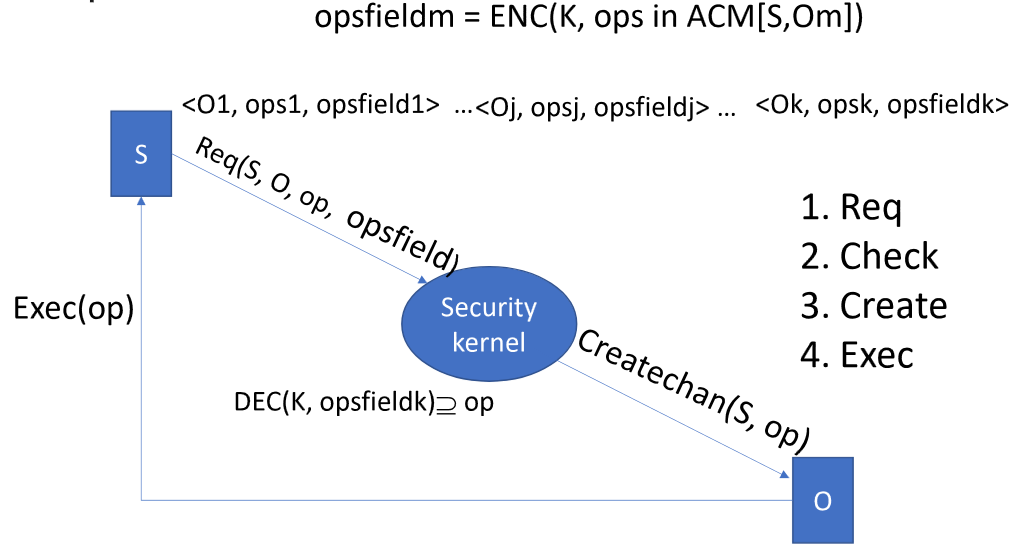
\includegraphics{images/challenge_2.png}
   \caption{Protocol schema}
   \label{fig:challenge_2}
\end{figure}

\subsection{Request}
Discover vulnerabilities in the proposed protocol or in the overall system under the assumption that there are no vulnerabilities in the encryption algorithm,
i.e. K cannnot be discovered because of  mathematical vulnerabilities.

\section{Proposed Solutions}
Below are listed possible vulnerabilities with some form of categorization,
although they may be related and/or not mutually exclusive.
\subsection{Vulnerability 1 - Authentication}

First of all we can observe that the lack of \textbf{authentication} allows an attacker to impersonate the \texttt{Security Kernel},
and thus to invoke \texttt{Createchan(S,op)} on objects, choosing arbitrarily \texttt{S} and \texttt{op} and the destination object.

% Besides, the attacker (\textit{subject} \texttt{A}), assuming he doesn't own a capability \texttt{C}, but owns a secret,
% may change the subject field in \texttt{Req(S,O,op,opsfield)},
% writing \texttt{S'} (subject who owns the desired capability \texttt{C}) 

\subsection{Vulnerability 2 - Integrity}
The attacker, by posing theirself inbetween entities {---}implementing a \textit{man-in-the-middle} attack{---},
may manipulate any field on any sent message,
with the exception of \texttt{opsfield}, since he cannot discover the secret \texttt{K}.

In this way he may achieve \textit{Denial-of-Service} or may obtain capabilities he does not own.
\nl

\begin{center}
   \textit{"Each subject manages a list with its own capabilities"}.
\end{center}
Depending on where and how such capabilities are stored and managed,
an attacker may manipulate them.

\subsection{Vulnerability 3 - Replay/Redirecting}

The attacker may sniff and record valid \texttt{Createchan(S,op)} and \texttt{Exec(op)} messages and replay them when desired.
Even if more costful and complex he may \textit{redirect}\footnote{equivalent to recording a message, dropping it, and replay it towards a different entity} them,
both obtaining access rights and denying the service for legitimate clients.

He may even copy \texttt{op} and \texttt{opsfield} and insert them in a \texttt{Req} sent by him.

\subsection{Vulnerability 4 - Overflow}

Probably not of interest here,
but every entity may be flooded by requests and messages,
resulting in the denial of service.